As mentioned in the previous section, the analytical solution is not practical
to use for most functions $f(x)$. Thus, we present a numerical solution to
approximate the analytical solution for the problem $Lu = f$.

\begin{subsection}{Description}
  Our solution is derived from the method of finite differences. We define
  a finite set of points on the interval $[0, 1]$ called the grid $D_h$ where
  the parameter $h$ is the size of the grid where a smaller $h$ denotes a finer
  grid. For our purposes, we consider $h=1/N$ for positive $N$ and
  create the uniform grid
  \begin{align}\label{uniform_grid}
    D_h = \{x_n| x_n = hn \text{ for $0 \leq n \leq N$}\}.
  \end{align}

  Define on this grid the discretized solution to the problem $Lu = f$ as
  \begin{align}\label{discretized_solution}
    [u]_h = \{u(x_n)\}.
  \end{align}
  Similarly, define the discretized function of $f(x)$ as $f^{(h)} = \{f(x_n)\}$.
  We wish to create a scheme $L_h$ that computes an approximate solution
  $u^{(h)} = \left\{u_0^{(h)}, u_1^{(h)}, \dots, u_N^{(h)}\right\}$ to the problem
  $Lu = f$, i.e.\ a scheme such that $L_h u^{(h)} = f^{(h)}$.

  Finding an approximation to $u''(x)$ should suggest how to construct
  the scheme $L_h$.
  To find an approximation for $u''(x)$, we investigate the Taylor expansion
  of $u(x+h)$ and $u(x-h)$ about $x$. These expansions are given by
  \begin{align*}
    u(x + h) &= u(x) + h u'(x) + \frac{h^2 u ''(x)}{2} + \frac{h^3 u^{(3)}(x)}{3!} + \frac{h^4 u^{(4)}(\xi_1)}{4!} \\
    u(x - h) &= u(x) - h u'(x) + \frac{h^2 u ''(x)}{2} - \frac{h^3 u^{(3)}(x)}{3!} + \frac{h^4 u^{(4)}(\xi_2)}{4!}
  \end{align*}
  where $x \leq \xi_1 \leq x + h$ and $x - h \leq \xi_2 \leq x$.
  Adding these two expressions and solving for $u''(x)$ shows that
  \begin{align}\label{second_deriv}
    u''(x) = \frac{u(x + h) - 2u(x) + u(x-h)}{h^2} - \frac{h^2(u^{(4)}(\xi_1) + u^{(4)}(\xi_2))}{4!}.
  \end{align}
  This suggests that we should define our numerical scheme by replacing $u''(x)$
  in $Lu = f$ with the approximation
  \[
  u''(x) \approx \frac{u(x + h) - 2u(x) + u(x-h)}{h^2}.
  \]
  Therefore, we define the numerical scheme as
  \begin{align}\label{numerical_scheme}
    L_h u^{(h)} = f^{(h)} :=
    \begin{cases}
      \frac{-u_{n+1} + 2 u_n - u_{n-1}}{h^2} + c u_n = f_n & \text{for $n= 1, \dots, N - 1$} \\
      u_0 = \epsilon \\
      u_N = \delta
    \end{cases}.
  \end{align}
  For $n=1,\dots,N-1$, the scheme presents us with the recurrence relation
  \[
  -u_{n-1} + (2 + ch^2) u_n - u_{n+1} = h^2 f_n
  \]
  with initial conditions $u_0 = \epsilon$ and $u_N = \delta$. This recurrence
  relation is represented by the following system of equations
  \begin{align*}
    (2 + ch^2) u_1 - u_2 &= h^2f_1 + u_0 \\
    -u_1 + (2 + ch^2) u_2 - u_3 &= h^2f_2 \\
    -u_2 + (2 + ch^2) u_3 - u_4 &= h^2f_3 \\
    \vdots &  \\
    -u_{N-2} + (2 + ch^2) u_{N-1} &= h^2f_{N-1} + u_N.
  \end{align*}
  In matrix form, this system of equations becomes
  \begin{align}\label{matrix_system}
    \begin{bmatrix}
      2 + ch^2 & -1 & 0 & \hdots & 0\\
      -1 & 2 + ch^2 & -1 & \hdots & 0\\
      0 & -1 & 2 + ch^2 & \hdots & 0\\
      \vdots & \vdots & \vdots & \ddots & \vdots \\
      0 & 0 & 0 & \hdots & 2+ch^2 \\
    \end{bmatrix}
    \begin{bmatrix}
      u_1 \\
      u_2 \\
      u_3 \\
      \vdots \\
      u_{N-1}
    \end{bmatrix}
    =
    \begin{bmatrix}
      h^2 f_1 + u_0 \\
      h^2 f_2 \\
      h^2 f_3 \\
      \vdots \\
      h^2 f_{N-1} + u_{N}
    \end{bmatrix}
  \end{align}
  The solution to this system of equations paired with the initial conditions
  allows us to explicitly find $u^{(h)}$, our scheme's solution.

  In section \ref{sec:scheme_prop} we examine the convergence, consistency,
  and stability of this scheme in order to determine its usefulness in
  approximating the analytical solution to the problem $Lu = f$.
\end{subsection}

\begin{subsection}{Implementation}
  In order to efficiently use the numerical scheme just described we will need to
implement the scheme using computational software.

\subsubsection{Discretized Solution}
We have implemented the numerical scheme described above in MATLAB which can be
used by calling the m-function \texttt{numerical\_scheme.m}. We will now
describe the parameters necessary to call the function, how the function
computes the solution, and the results outputted by the function. Please refer
to appendix \ref{append_analytical} for the function definition in MATLAB.

This m-function requires the following parameters to compute the numerical solution:
\begin{itemize}
  \item \texttt{f} - MATLAB function that represents the function $f$ in the differential equation $Lu = f$.
  \item \texttt{c} - A real number that represents the constant $c$ in the differential equation $Lu = f$.
  \item \texttt{initials} - An array with two elements representing the initial conditions in the problem
    $Lu=f$. The first element of the array is $\epsilon$ and the second element of the array is $\delta$.
  \item \texttt{interval} - An array with two elements representing the endpoints of the interval of definition in
    the problem $Lu = f$.
  \item \texttt{subintervals} - An integer that represents the number of subintervals with which to construct
    the uniform nodes on the interval of definition. This corresponds to an
    $h$-value of $1/\texttt{subintervals}$ on the grid $D_h$.
\end{itemize}

Calling the function as follows
\[
  \texttt{numerical\_scheme(f, c, initials, interval, subintervals)}
\]
returns the array \texttt{[x, u]} where \texttt{x} is an array whose elements are
the nodes on the grid $D_h$ and \texttt{u} is an array whose elements are the
numerical solution obtained by the scheme $L_h u^{(h)} = f^{(h)}$ evaluated on the
nodes of the grid.

From these parameters, after verifying that $c$ is a positive real number,
the function creates and assigns to \texttt{x} the uniform
nodes equally spaced on the passed interval with width 1/\texttt{subintervals}. We then
construct the  coefficient matrix \texttt{A} and the right-hand side vector \texttt{b} of the equation
in \eqref{matrix_system}. Finally, we then assign to \texttt{u} the solution vector
which is given by \texttt{initials(1), A\textbackslash b, initials(2)}.

Using this function then allows us to compute the numerical solution to the problem
$Lu = f$.

\subsubsection{Plotting}
Now that we have an implementation to compute the numerical approximation to the
exact solution to the problem $Lu =f$, we would like to also have a way to plot
that solution.

In order to achieve that goal, we have implemented a function that performs
linear spline interpolation where the interpolants are the values of the computed
approximate solution using the numerical scheme $L_h u^{(h)} = f^{(h)}$.

The m-function \texttt{plot\_interpolation.m} takes as input the output from the
m-function \texttt{numerical\_scheme.m}, i.e.\ the nodes \texttt{x} and the
solution vector \texttt{u}. This produces a figure that plots the original
vector \texttt{u} and the linear splines that interpolate the elements of the
vector \texttt{u}.

As the number of nodes increases, the plot of the solution becomes smoother as
can be seen in Figure \ref{example_plot}.

\begin{figure}[h!]
  \begin{center}
    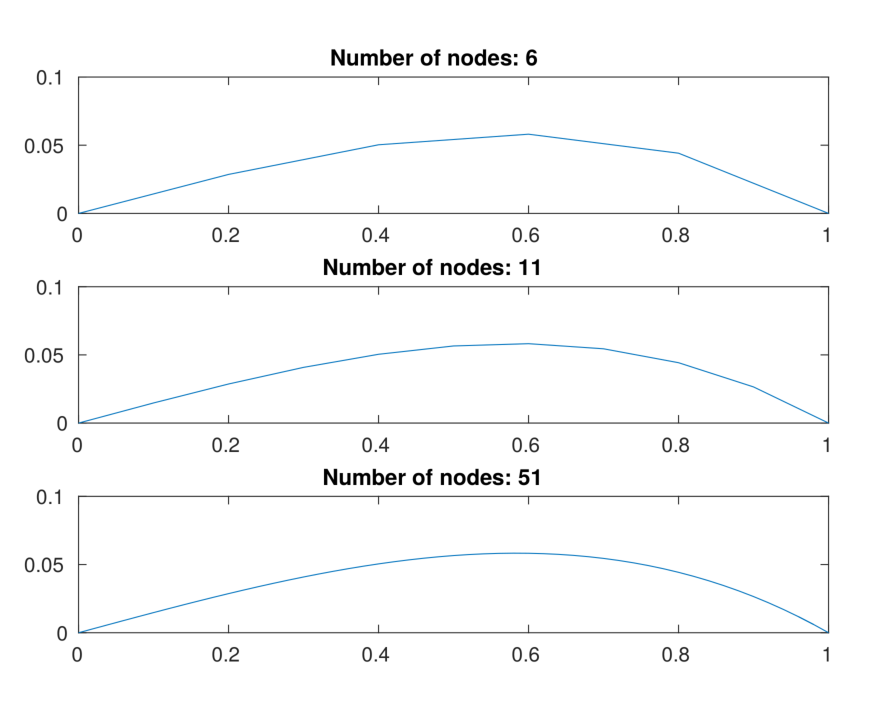
\includegraphics[scale=0.75]{example}
  \end{center}
  \caption{Plotted solution obtained from numerical scheme $L_h u^{(h)} = f^{(h)}$ for the problem $Lu = f$ with
    $f(x) = x$, $c =1$, and initial conditions $u(0) = 0$, $u(1) = 0$ for increasing number of nodes
    using the function \texttt{plot\_interpolation.m}.}\label{example_plot}
\end{figure}

We also have provided the m-function \texttt{linear\_interpolation.m} that evaluates
the solution obtained from the m-function \texttt{numerical\_scheme.m} for any $x$
on the interval of definition for the problem $Lu = f$. This is achieved
by evaluating the linear spline that interpolates the two nodes that contain
the point $x$ and returning that value.

The function definitions for \texttt{plot\_interpolation.m} and \texttt{linear\_interpolation.m}
can be found in Appendix \ref{append_plot}.
\end{subsection}
